%File: formatting-instructions-latex-2023.tex
%release 2023.0
\documentclass[letterpaper]{article} % DO NOT CHANGE THIS
\usepackage{aaai23}  % DO NOT CHANGE THIS
\usepackage{times}  % DO NOT CHANGE THIS
\usepackage{helvet}  % DO NOT CHANGE THIS
\usepackage{courier}  % DO NOT CHANGE THIS
\usepackage[hyphens]{url}  % DO NOT CHANGE THIS
\usepackage{graphicx} % DO NOT CHANGE THIS
\urlstyle{rm} % DO NOT CHANGE THIS
\def\UrlFont{\rm}  % DO NOT CHANGE THIS
\usepackage{natbib}  % DO NOT CHANGE THIS AND DO NOT ADD ANY OPTIONS TO IT
\usepackage{caption} % DO NOT CHANGE THIS AND DO NOT ADD ANY OPTIONS TO IT
\frenchspacing  % DO NOT CHANGE THIS
\setlength{\pdfpagewidth}{8.5in}  % DO NOT CHANGE THIS
\setlength{\pdfpageheight}{11in}  % DO NOT CHANGE THIS
%
% These are recommended to typeset algorithms but not required. See the subsubsection on algorithms. Remove them if you don't have algorithms in your paper.
\usepackage{algorithm}
\usepackage{algorithmic}
\usepackage{caption}
\captionsetup[figure]{font=small}
\captionsetup[table]{font=small}
\usepackage{subcaption}
\usepackage{multirow}
\usepackage{xspace}
\usepackage{makecell}
\usepackage{verbatim}
%\usepackage{caption}
%\usepackage{subcaption}

% new add package
\usepackage[utf8]{inputenc} % allow utf-8 input
\usepackage[T1]{fontenc}    % use 8-bit T1 fonts
\usepackage{url}            % simple URL typesetting
\usepackage{booktabs}       % professional-quality tables
\usepackage{amsfonts}       % blackboard math symbols
\usepackage{nicefrac}       % compact symbols for 1/2, etc.
\usepackage{microtype}      % microtypography
\usepackage{bm}
\usepackage{enumitem}
\usepackage{graphicx}
\usepackage{amsmath}
%\usepackage{subfigure}
% \usepackage[numbers, sort]{natbib}
% \usepackage[round]{natbib}
% \usepackage[round]{natbib}
\usepackage{caption}
\captionsetup[figure]{font=small}
\captionsetup[table]{font=small}
\usepackage{algorithm}
% \usepackage{appendix}
\usepackage{algorithmic}
\usepackage[dvipsnames]{xcolor}
% \newtheorem{example}{Example} 
% \usepackage{wrapfig}
\newtheorem{theorem}{Theorem}
\newtheorem{lemma}[theorem]{Lemma} 
\newtheorem{proposition}[theorem]{Proposition} 
\newtheorem{remark}[theorem]{Remark}
\newtheorem{corollary}[theorem]{Corollary}
\newtheorem{definition}[theorem]{Definition}
\newtheorem{conjecture}[theorem]{Conjecture}
\newtheorem{axiom}[theorem]{Axiom}
\usepackage{enumitem}
\DeclareMathOperator*{\argmin}{arg\,min}
\DeclareMathOperator*{\argmax}{arg\,max}
%\usepackage[colorlinks=true,bookmarksopen,pdfsubject={algorithms},linkcolor={MidnightBlue}, anchorcolor={black}, citecolor={MidnightBlue}, filecolor={magenta}, menucolor={black}, pagecolor={red},backref=none,urlcolor={MidnightBlue}]{hyperref}
\usepackage[colorlinks=true,bookmarksopen,pdfsubject={algorithms},linkcolor={MidnightBlue}, anchorcolor={black}, citecolor={MidnightBlue}, filecolor={magenta}, menucolor={black}, pagecolor={red},backref=none,urlcolor={MidnightBlue}]{hyperref}
\usepackage{array}
\usepackage{multirow}
\usepackage{wrapfig,lipsum,booktabs}
% These are are recommended to typeset listings but not required. See the subsubsection on listing. Remove this block if you don't have listings in your paper.
\usepackage{newfloat}
\usepackage{listings}
\lstset{%
	basicstyle={\footnotesize\ttfamily},% footnotesize acceptable for monospace
	numbers=left,numberstyle=\footnotesize,xleftmargin=2em,% show line numbers, remove this entire line if you don't want the numbers.
	aboveskip=0pt,belowskip=0pt,%
	showstringspaces=false,tabsize=2,breaklines=true}
\floatstyle{ruled}
\newfloat{listing}{tb}{lst}{}
\floatname{listing}{Listing}
%
% Keep the \pdfinfo as shown here. There's no need
% for you to add the /Title and /Author tags.
\pdfinfo{
/TemplateVersion (2023.1)
}

% DISALLOWED PACKAGES
% \usepackage{authblk} -- This package is specifically forbidden
% \usepackage{balance} -- This package is specifically forbidden
% \usepackage{color (if used in text)
% \usepackage{CJK} -- This package is specifically forbidden
% \usepackage{float} -- This package is specifically forbidden
% \usepackage{flushend} -- This package is specifically forbidden
% \usepackage{fontenc} -- This package is specifically forbidden
% \usepackage{fullpage} -- This package is specifically forbidden
% \usepackage{geometry} -- This package is specifically forbidden
% \usepackage{grffile} -- This package is specifically forbidden
% \usepackage{hyperref} -- This package is specifically forbidden
% \usepackage{navigator} -- This package is specifically forbidden
% (or any other package that embeds links such as navigator or hyperref)
% \indentfirst} -- This package is specifically forbidden
% \layout} -- This package is specifically forbidden
% \multicol} -- This package is specifically forbidden
% \nameref} -- This package is specifically forbidden
% \usepackage{savetrees} -- This package is specifically forbidden
% \usepackage{setspace} -- This package is specifically forbidden
% \usepackage{stfloats} -- This package is specifically forbidden
% \usepackage{tabu} -- This package is specifically forbidden
% \usepackage{titlesec} -- This package is specifically forbidden
% \usepackage{tocbibind} -- This package is specifically forbidden
% \usepackage{ulem} -- This package is specifically forbidden
% \usepackage{wrapfig} -- This package is specifically forbidden
% DISALLOWED COMMANDS
% \nocopyright -- Your paper will not be published if you use this command
% \addtolength -- This command may not be used
% \balance -- This command may not be used
% \baselinestretch -- Your paper will not be published if you use this command
% \clearpage -- No page breaks of any kind may be used for the final version of your paper
% \columnsep -- This command may not be used
% \newpage -- No page breaks of any kind may be used for the final version of your paper
% \pagebreak -- No page breaks of any kind may be used for the final version of your paperr
% \pagestyle -- This command may not be used
% \tiny -- This is not an acceptable font size.
% \vspace{- -- No negative value may be used in proximity of a caption, figure, table, section, subsection, subsubsection, or reference
% \vskip{- -- No negative value may be used to alter spacing above or below a caption, figure, table, section, subsection, subsubsection, or reference

\setcounter{secnumdepth}{0} %May be changed to 1 or 2 if section numbers are desired.

% The file aaai23.sty is the style file for AAAI Press
% proceedings, working notes, and technical reports.
%

% Title

% Your title must be in mixed case, not sentence case.
% That means all verbs (including short verbs like be, is, using,and go),
% nouns, adverbs, adjectives should be capitalized, including both words in hyphenated terms, while
% articles, conjunctions, and prepositions are lower case unless they
% directly follow a colon or long dash
% \title{AAAI Press Formatting Instructions \\for Authors Using \LaTeX{} --- A Guide}
% \author{
%     %Authors
%     % All authors must be in the same font size and format.
%     Written by AAAI Press Staff\textsuperscript{\rm 1}\thanks{With help from the AAAI Publications Committee.}\\
%     AAAI Style Contributions by Pater Patel Schneider,
%     Sunil Issar,\\
%     J. Scott Penberthy,
%     George Ferguson,
%     Hans Guesgen,
%     Francisco Cruz\equalcontrib,
%     Marc Pujol-Gonzalez\equalcontrib
% }
% \affiliations{
%     %Afiliations
%     \textsuperscript{\rm 1}Association for the Advancement of Artificial Intelligence\\
%     % If you have multiple authors and multiple affiliations
%     % use superscripts in text and roman font to identify them.
%     % For example,

%     % Sunil Issar, \textsuperscript{\rm 2}
%     % J. Scott Penberthy, \textsuperscript{\rm 3}
%     % George Ferguson,\textsuperscript{\rm 4}
%     % Hans Guesgen, \textsuperscript{\rm 5}.
%     % Note that the comma should be placed BEFORE the superscript for optimum readability

%     1900 Embarcadero Road, Suite 101\\
%     Palo Alto, California 94303-3310 USA\\
%     % email address must be in roman text type, not monospace or sans serif
%     publications23@aaai.org
% %
% % See more examples next
% }

% %Example, Single Author, ->> remove \iffalse,\fi and place them surrounding AAAI title to use it
% \iffalse
% \title{My Publication Title --- Single Author}
% \author {
%     Author Name
% }
% \affiliations{
%     Affiliation\\
%     Affiliation Line 2\\
%     name@example.com
% }
% \fi

% \iffalse
%Example, Multiple Authors, ->> remove \iffalse,\fi and place them surrounding AAAI title to use it
\title{Accelerating Inverse Learning via Intelligent Localization with \\ Exploratory Sampling}
\author {
    % Authors
    Jiaxin Zhang\textsuperscript{\rm 1},
    Sirui Bi\textsuperscript{\rm 2},
    Victor Fung\textsuperscript{\rm 3}
}
\affiliations {
    % Affiliations
    \textsuperscript{\rm 1} Intuit AI Research \\ 
    \textsuperscript{\rm 2} Walmart Global Tech \\ 
    \textsuperscript{\rm 3} Georgia Institute of Technology\\
    jiaxin\_zhang@intuit.com, sirui.bi@walmart.com, victorfung@gatech.edu \\
}
%\fi


% REMOVE THIS: bibentry
% This is only needed to show inline citations in the guidelines document. You should not need it and can safely delete it.
\usepackage{bibentry}
% END REMOVE bibentry

\begin{document}

\maketitle

\begin{abstract}
In the scope of ``AI for Science'', solving inverse problems is a longstanding challenge in materials and drug discovery, where the goal is to determine the hidden structures given a set of desirable properties. Deep generative models are recently proposed to solve inverse problems, but these currently use expensive forward operators and struggle in precisely localizing the exact solutions and fully exploring the parameter spaces without missing solutions. In this work, we propose a novel approach (called {iPage}) to accelerate the inverse learning process by leveraging probabilistic inference from deep invertible models and deterministic optimization via fast gradient descent. Given a target property, the learned invertible model provides a posterior over the parameter space; we identify these posterior samples as an intelligent prior initialization which enables us to narrow down the search space. We then perform gradient descent to calibrate the inverse solutions within a local region. Meanwhile, a space-filling sampling is imposed on the latent space to better explore and capture all possible solutions. We evaluate our approach on three benchmark tasks and two created datasets with real-world applications from quantum chemistry and additive manufacturing, and find our method achieves superior performance compared to several state-of-the-art baseline methods. The iPage code is available at \url{https://github.com/jxzhangjhu/MatDesINNe}.
\end{abstract}

\section{Introduction}
\label{intro}

A fundamental problem in materials and drug discovery is to find novel structures (e.g., molecules or crystals) with desirable properties. One typical approach is to search in the chemical space based on a specific property prediction. Inverse design provides a promising way for this problem by inverting this paradigm by starting with the desired functionality and searching for an ideal molecular structure \citep{sanchez2018inverse, yao2021inverse}, as opposed to the direct approach that maps from existing molecules in chemical space to the properties. Mathematically speaking, inverse design tries to solve a nonlinear inverse problem, which remains a significant challenge in natural sciences and mathematics, and also plays a critical role in safe decision-making with uncertainty. Typically, the approach is to develop a mathematical operator or physical model $\Omega$ on how measured observations (e.g., properties) $\mathbf{y} \in \mathbb{R}^{M}$ arise from the input hidden parameters (e.g., chemical space) $\mathbf{x} \in \mathbb{R}^D$ and such mapping $\mathbf{y}=\Omega(\mathbf{x})$ represents the {\em forward process}. The opposite direction, the {\em inverse process} $\mathbf{x} = \Omega^{-1}(\mathbf{y})$, involves the inference of the hidden parameters from measurements. However, the inverse process is ill-posed with a one-to-many mapping such that finding $\Omega^{-1}$ becomes intractable. 

Unfortunately, inverse design in scientific exploration differs from conventional inverse problems in that it poses several unique additional challenges. First, \emph{the forward operator $\Omega$ is not explicitly known}. In many cases, the forward operator is modeled by first-principles calculations or large-scale complex simulations \cite{lavin2021simulation}, including molecular dynamics and density functional theory \cite{liu2022machine}. This challenge makes inverse design difficult to leverage recent advances in solving inverse problems, such as MRI reconstruction \citep{wang2020deep}, implanting on images through generative models with large datasets \citep{asim2020invertible}. Second, \emph{the search space $\mathbf{x} \in \mathbb{R}^D$ is often huge}. For example, small drug-like molecules have been estimated to contain between 10\textsuperscript{23} to 10\textsuperscript{60} unique cases 
\citep{ertl2009estimation}, while solid materials have an even larger space. This challenge results in obvious obstacles for using global search via Bayesian optimization or using Bayesian inference via Markov Chain Monte Carlo (MCMC) since either method is prohibitively slow for high-dimensional inverse problems \cite{zhang2019learning}. Third, \emph{multimodal solutions have a one-to-many mapping issue}. In other words, there are multiple solutions that match the desirable property. This issue leads to difficulties in pursuing all possible solutions through a gradient-based optimization, which converges a single deterministic solution and is easily trapped into local minima \cite{zhang2021enabling}. Probabilistic inference also has limitations in approximating complex posteriors, which may cause the simple point estimates (e.g., maximum a posterior (MAP)) to have misleading solutions \citep{sun2020deep}. This work aims at addressing these challenges by leveraging advantages from probabilistic inference and deterministic optimization to accelerate solving of generic inverse problems. The key insight is to first learn an approximate posterior distribution by training an invertible neural network (INN) given paired datasets $\mathcal{D} = \{\mathbf{x}_i, \mathbf{y}_i \}_{i=1}^m$ and then perform a local search via optimization by starting with these posterior samples as good initialization (called ``intelligent priors''). 

Specifically, we propose a dynamic bi-directional training scheme to obtain a backward model and a forward model simultaneously. The backward model is used to generate posterior samples $\mathbf{x}^*$ given target properties $\mathbf{y}^*$. These posterior samples $\mathbf{x}^*$ as intelligent priors significantly narrow down the search space from the entire domain to a local domain. The forward model serves as a surrogate of the forward operator $\Omega$ and provides an accurate gradient estimate with respect to the design space $\mathbf{x} \in \mathbb{R}^D$ via automatic differentiation. This enables us to localize all possible solutions simultaneously by conducting an efficient gradient-based optimization starting from the intelligent priors $\mathbf{x}^*$. Unlike direct global search with random initialization, our method significantly accelerates inverse learning by conducting an efficient local search via gradient descent on low-dimensional design space. Compared with probabilistic inference via unsupervised generative models, our inverse solutions are closer to the ground truth since a supervised localization scheme is performed on the posterior samples. Our method is also applicable to high-dimensional problems with relatively small datasets given an expensive forward operator $\Omega$. More importantly, we propose an exploratory sampling strategy with an enhanced space-filling capability to better explore and capture all possible solutions in the design space. To the best of our knowledge, this is the \emph{first work} to investigate space-filling sampling on the latent variable of the INN model to improve sampling exploration with variance reduction. As a result, we achieve superior performance in re-simulation accuracy, space exploration, and solution diversity through multiple artificial benchmarks. We also curate two real-world datasets from quantum chemistry and additive manufacturing and create a set of physically meaningful tasks and metrics for the problem of inverse learning. We find our method achieves superior performance compared to several state-of-the-art baseline methods.

\section{Related Work}
{\bf Bayesian and Variational Approaches.}
From the inference perspective, solving inverse problems can be achieved by estimating the full posterior distributions of the parameters conditioned on a target property. Bayesian methods, such as approximate Bayesian computing \citep{yang2018predictive}, are ideal choices to model the conditional posterior but this idea still encounters various computational challenges in high-dimensional cases \cite{zhang2018effect,zhang2018quantification}. An alternative choice are variational approaches, e.g., conditional GANs \citep{wang2018high} and conditional VAEs \citep{sohn2015learning}, which enable the efficient approximation of the true posterior by learning the transformation between latent variables and parameter variables. However, the direct application of both conditional generative models for inverse problems is challenging because a large dataset is often required \citep{tonolini2020variational}.

\vspace{0.2cm}
\noindent {\bf Deep Generative Models.} 
Many recent efforts have been made on solving inverse problems via deep generative models \citep{asim2020invertible, whang2021composing, whang2021solving, daras2021intermediate, sun2020deep, kothari2021trumpets,song2021solving}. For example, \citet{asim2020invertible} focuses on producing a point estimate motivated by the MAP formulation and \cite{whang2021composing} aims at studying the full distributional recovery via variational inference. A follow-up study from \cite{whang2021solving} is to study image inverse problems with a normalizing flow prior. For MRI or implanting on images, strong baseline methods exist that benefit from explicit forward operator \citep{sun2020deep, asim2020invertible, kothari2021trumpets}. We do not expect any benefit from using our method here. Instead, our focus is on the inverse design perspective where paired data $\mathcal{D} = \{\mathbf{x}_i, \mathbf{y}_i \}_{i=1}^m$ is limited since the forward operator is not explicitly known and is often computationally intensive. 

\vspace{0.2cm}
 \noindent{\bf Invertible Models.} 
Flow-based models \citep{rezende2015variational,dinh2016density,kingma2018glow,grathwohl2018ffjord,wu2020stochastic,nielsen2020survae}, may offer a promising direction to infer the posterior by training on invertible architectures. Some recent studies have leveraged this unique property of invertible models to address several challenges in solving inverse problems \citep{ardizzone2018analyzing, kruse2021benchmarking}. However, these existing invertible model approaches suffer from limitations \citep{ren2020benchmarking} in fully exploring the parameter space, leading to missed potential solutions, and often fail to precisely localize the optimal solutions due to noisy solutions and inductive errors, specifically in materials design problems \cite{fung2021inverse,fung2022atomic}.  

\vspace{0.2cm}
\noindent{\bf Surrogate-based Optimization.}
Another approach is to build a neural network surrogate and then conduct surrogate-based optimization via gradient descent. This is common in scientific and engineering applications \citep{forrester2009recent, gomez2018automatic, white2019multiscale}. The essential challenge is that the forward model is often time-consuming so a faster surrogate enables an intractable search. A recent study in the scope of surrogate-based optimization is the neural-adjoint (NA) method \citep{ren2020benchmarking} which directly searches the global space via gradient descent starting from random initialization, such that a large number of interactions are required to converge and its solutions are easily trapped in the local minima \citep{deng2021neural}. Although the neural-adjoint (NA) method boosts the performance by down-selecting the top solutions from multiple starts, the computational cost is significantly high, specifically for high-dimensional problems. 

\section{Methodology}
\subsection{Augmented Inverse Learning Formulation}
\begin{figure}[!h]
  \centering
  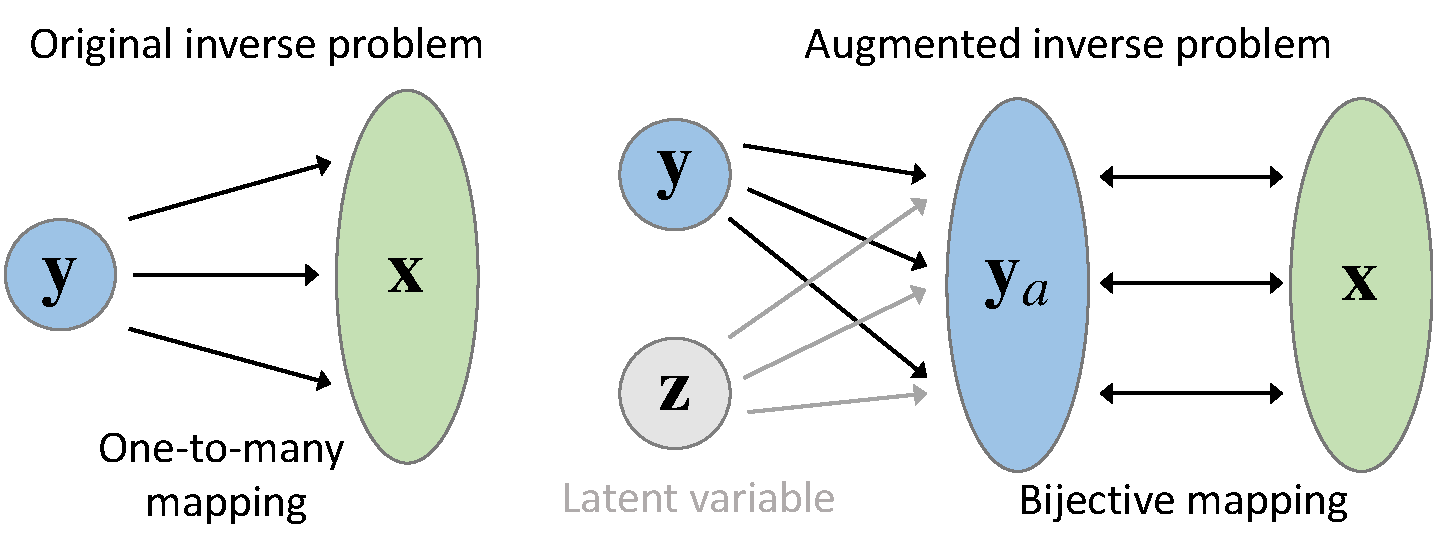
\includegraphics[width=0.95\linewidth]{inverse_aug2.pdf}
  \caption{Original inverse problem often encounters the ill-posed issue due to one-to-many mappings. An augmented inverse problem is formulated based on bijective mapping with additional latent variable $\mathbf{z}$.}
\label{fig:eq_bijectiv}
  \vspace{-6mm}
\end{figure}

In natural sciences, a mathematical or physical model is often developed to describe how measured observations $\mathbf{y} \in \mathbb{R}^{M}$ arise from the hidden parameters $\mathbf{x} \in \mathbb{R}^D$, to yield such a mapping $\mathbf{y}=\Omega(\mathbf{x})$. To completely capture all possible inverse solutions given observed measurements, a proper inverse model should enable the estimation of the full posterior distribution $p(\mathbf{x}|\mathbf{y})$ of hidden parameters $\mathbf{x}$ conditioned on an observation $\mathbf{y}$. One promising approach is to approximate $p(\mathbf{x}|\mathbf{y})$ with a tractable probabilistic model $\hat{p}(\mathbf{x}|\mathbf{y})$ by leveraging the advantage of the flexibility to generate paired training data $\left\{(\mathbf{x}_i, \mathbf{y}_i)_{i=1}^N \right\}$ from the well-understood forward process $\mathbf{y}_i = \Omega(\mathbf{x}_i)$. Invertible neural networks (INNs) \citep{ rezende2015variational,dinh2016density,ardizzone2018analyzing} can be trained in the forward process and then used in the invertible mode to sample from $p(\mathbf{x}|\mathbf{y})$ for any specific $\mathbf{y}$. This is achieved by adding a latent variable $\mathbf{z} \in \mathbb{R}^K$, which encodes the inherent information loss in the forward process. In other words, the latent variable $\mathbf{z}$ drawn from a Gaussian distribution $p(\mathbf{z}) = \mathcal{N}(0,I_K)$ is able to encode the intrinsic information about $\mathbf{x}$ that is {\em not} contained in $\mathbf{y}$. To this end, an augmented inverse problem is formulated based on such a bijective mapping (Fig. \ref{fig:eq_bijectiv}):
\begin{equation}
    % f_a(\mathbf{x}) = \mathbf{y}_a = [\mathbf{y};\mathbf{z}], \textnormal{with} 
    % \mathbf{x} = f^{-1}(\mathbf{y}) = f^{-1}_a(\mathbf{y}_a) = f^{-1}_a(\mathbf{y},\mathbf{z}), \quad \mathbf{z} \sim p(\mathbf{z}). 
    % \mathbf{x} = f^{-1}(\mathbf{y}) = h(\mathbf{y}_a) = h(\mathbf{y},\mathbf{z}), \quad \mathbf{z} \sim p(\mathbf{z})
    \mathbf{x} = h(\mathbf{y}_a; \phi) = h(\mathbf{y},\mathbf{z}; \phi), \quad \mathbf{z} \sim p(\mathbf{z}) \label{eq:bijective}
\end{equation}
where $h$ is a function of $\mathbf{y}$ and $\mathbf{z}$, parametrized by an INN with parameters $\phi$. Forward training optimizes the mapping $\mathbf{x} \rightarrow \mathbf{y}_a = [\mathbf{y}, \mathbf{z}]$ and implicitly determines the inverse mapping $\mathbf{x} = h(\mathbf{y},\mathbf{z})$. In the context of INNs, the posterior distribution $p(\mathbf{x}|\mathbf{y})$ is represented by the deterministic function $\mathbf{x}=h(\mathbf{y},\mathbf{z})$ that transforms the known probability distribution $p(\mathbf{z})$ to parameter $\mathbf{x}$-space, conditional on measurements $\mathbf{y}$. Thus, given a chosen observation $\mathbf{y}^*$ with the learned $h$, we can obtain the posterior samples $\mathbf{x}_k$ which follows the posterior distribution $p(\mathbf{x} | \mathbf{y}^*)$ via a transformation $\mathbf{x}_k = h(\mathbf{y}^*,\mathbf{z}_k)$ with prior samples drawn from $\mathbf{z}_k \sim p(\mathbf{z})$.

The invertible architecture simultaneously learns the model $h(\mathbf{y},\mathbf{z}; \phi)$ of the inverse process jointly with a model $f(\mathbf{x};\phi)$ which approximates the true forward process $\Omega(\mathbf{x})$:
\begin{equation}
    [\mathbf{y},\mathbf{z}] = f(\mathbf{x};\phi) = [f_{\mathbf{y}}(\mathbf{x};\phi), f_{\mathbf{z}}(\mathbf{x};\phi)] = h^{-1}(\mathbf{x};\phi)
\end{equation}
where $f_{\mathbf{y}}(\mathbf{x};\phi) \approx \Omega(\mathbf{x})$, model $f$ and $h$ share the same parameters $\phi$ in a single invertible neural network. Therefore, our approximated posterior model $\hat{p}(\mathbf{x}|\mathbf{y})$ is built into the invertible neural network representation
\begin{equation}
    \hat{p}(\mathbf{x} = h(\mathbf{y},\mathbf{z}; \phi) | \mathbf{y}) = p(\mathbf{z})/ \left| \bm J_{\mathbf{x}} \right| 
\end{equation}
where the Jacobian $\bm J_{\mathbf{x}}$ can be efficiently computed by using neural spline flows \citep{durkan2019neural}. 

\subsection{Dynamical Bi-directional Training}
To optimize the loss more effectively, we perform a dynamic bi-directional training scheme by accumulating gradients from both forward and backward directions before updating the parameters, using an adaptive update strategy for the forward and backward loss weights $\lambda$. Specifically, the INN training is performed by minimizing the total loss:
\begin{equation}
    \mathcal{L}_{\textit{total}} = \lambda_x \mathcal{L}_{x} +  \lambda_y \mathcal{L}_{y} + \lambda_z \mathcal{L}_{z} \label{eq:total_loss}
\end{equation}
where $\mathcal{L}_{y}$ is a forward supervised loss that matches the neural network prediction $f_{\mathbf{y}}(\mathbf{x}_k;\phi)$ to the true observation via known forward simulation $\mathbf{y}_k = \Omega(\mathbf{x}_k)$.
\begin{equation}
    \mathcal{L}_{y} = \sum_{k=1}^N || f_{\mathbf{y}}(\mathbf{x}_k;\phi) - \mathbf{y}_k  ||^2. \label{eq:loss_y}
\end{equation}
$\mathcal{L}_z$ is an unsupervised loss for the latent variable, which penalizes deviations between the joint distribution $\hat{p}(\mathbf{y} = f_{\mathbf{y}}(\mathbf{x}),\mathbf{z}=f_{\mathbf{z}}(\mathbf{x}))$ and the product of the latent distribution $p(\mathbf{z})$ and the marginal distributions of $p(\mathbf{y}=\Omega(\mathbf{x}))$:
\begin{equation}
    \mathcal{L}_{z} = \textup{MMD}\left\{f(\mathbf{x}_k; \phi); p(\mathbf{y}) p(\mathbf{z})) \right\} \label{eq:loss_z}
\end{equation}
where MMD refers to the Maximum Mean Discrepancy \citep{gretton2012kernel,gretton2012optimal}, a kernel-based approach that only requires samples from each probability distribution to be compared. Practically, $\mathcal{L}_{z}$ enforces $\mathbf{z}$ follow the desired Gaussian distribution $p(\mathbf{z})$, and ensures $\mathbf{z}$ and $\mathbf{y}$ are independent without sharing the same information. 

$\mathcal{L}_{\mathbf{x}}$ is an unsupervised loss, which is implemented by MMD and used to penalize the mismatch between the distribution of backward predictions and the prior data distribution $p(\mathbf{x})$ if it is known,
\begin{equation}
   \mathcal{L}_{\mathbf{x}} = \textup{MMD}\left\{f^{-1}(\mathbf{y}_k, \mathbf{z}_k; \phi), p(\mathbf{x}) \right\}  \label{eq:loss_x}
\end{equation}
where $\mathcal{L}_{\mathbf{x}}$ aims to improve convergence and does not interfere with optimization. Theoretically, if $\mathcal{L}_{\mathbf{y}}$ and $\mathcal{L}_{\mathbf{z}}$ has converged to zero, and $\mathcal{L}_{\mathbf{x}}$ is guaranteed to be zero so that the samples drawn from Eq.~\eqref{eq:bijective} will follow the true posterior $p(\mathbf{x}|\mathbf{y}^*)$ for any observation $\mathbf{y}^*$. Therefore, a point estimate from the true posterior will lead to an exact inverse solution. However, practically, due to a finite training time, there is always a difference between the $\mathcal{L}_{\textup{total}}$ and zero loss, as well as a residual dependency between $\mathbf{y}$ and $\mathbf{z}$. This causes a mismatch between the approximated posterior $\hat{p}(\mathbf{x}|\mathbf{y})$ and the true posterior $p(\mathbf{x}|\mathbf{y})$. 

Our objective is to minimize the mismatch by optimization with a good initialization. Assuming $n_{t}$ training epochs are used, we set an initial large weight for the supervised loss $\lambda_{\mathbf{y}}^i \rightarrow N_{\ell}, i =1,...,n_t/2, \ N_{\ell} \gg 1$ to seek an accurate regression model $f_{\mathbf{y}}(\mathbf{x};\phi)$ and then perform an adaptive decay when $i = n_t/2,..,n_t$ and ensure $\lambda_{\mathbf{y}}^{n_t} \rightarrow 0$ at the end of training. The model with minimal $\ell_2$ loss $f_{\mathbf{y}}(\mathbf{x};\phi^*)$ is saved for prediction and gradient estimation. Meanwhile, the weights of unsupervised loss $\lambda_{\mathbf{x}}$ and $\lambda_{\mathbf{z}}$ are set by $\lambda_{\mathbf{x}}^i \rightarrow 0$ and $\lambda_{\mathbf{z}}^i \rightarrow 0$ when $i=1,...,n_t/2$ and are then adaptively increased until $\lambda_{\mathbf{x}}^{n_t} \rightarrow N_{\ell}$ and $\lambda_{\mathbf{z}}^{n_t} \rightarrow N_{\ell}$ where we minimize the residual dependency between $\mathbf{y}$ and $\mathbf{z}$ to approximate the true posterior  $p(\mathbf{x}|\mathbf{y})$. To do so, the backward MMD loss is minimized such that the learned posterior will be closer to the true posterior. 
\begin{figure*}[h!]
\vspace{-0.2cm}
    \centering
    \includegraphics[width=0.99\textwidth]{iPage1.pdf}
    \vspace{-0.2cm}
    \caption{{Localizing inverse solutions from intelligent priors (posterior samples)}. The approximated posterior and its MAP estimator both deviate from the exact solution but successfully narrow down the search space. Our objective is to localize the exact solution by leveraging these posterior samples as intelligent initialization such that the process can be accelerated.}
    \label{fig:localize}
% \vspace{-0.3cm}
\end{figure*}

\subsection{Localization from Posterior Samples}
After finishing the dynamic bi-directional training, a set of posterior samples can be drawn from the approximated posterior distribution $\hat{p}(\mathbf{x}|\mathbf{y})$, as the orange dots shown in Fig. \ref{fig:localize} (left). Compared with the prior distribution $p(\mathbf{x})$, these posterior samples drawn from ${p}(\mathbf{x}|\mathbf{y})$ in either are able to reduce the search space with a smaller gap from the exact solution, which fits both unimodal and multimodal scenarios. Instead of global random search used by surrogate-based optimization, we localize the solutions starting from these posterior samples which can be seen as \emph{intelligent priors} (see Fig. \ref{fig:localize} (right)) and the smaller gap can be quickly filled by gradient descent with few steps. The local search via optimization would significantly accelerate the localization process and decrease the risk of local minima in global random search. This novel idea mainly consists of three steps: 

\begin{itemize}[leftmargin=10pt]
    \item {\bf Step 1 (Prior Exploration)}: Given a specific target $\hat{\mathbf{y}}$, repeat for a latent sample $\left\{\mathbf{z}_i \sim p(\mathbf{z}) \right\}_{i=1}^m$ to obtain a posterior sample $\left\{\hat{\mathbf{x}}_i \sim \hat{p}({\mathbf{x}} | \hat{\mathbf{y}}) \right\}_{i=1}^m$ which can be interpreted as a prior exploration of the solution space. Compared to the samples $\mathbf{x}_i$ directly drawn from the prior distribution $p(\mathbf{x})$, these posterior samples $\hat{\mathbf{x}}_i$ serve as good initialization, significantly shorten the distance to the exact inverse solution, as explained in Fig. \ref{fig:localize} (a) and (b). 
    \item {\bf Step 2 (Gradient Estimation)}: Extract the saved regression model $\hat{f}_{\mathbf{y}}(\mathbf{x};{\phi}^*)$ where the neural network parameters ${\phi}^*$ are fixed, and evaluate the model only by changing the input $\mathbf{x}$ to the network. The gradient at the current input $\hat{\mathbf{x}}_i$ can be defined as
    \begin{equation}
        \mathbf{g}_i = \frac{\partial\mathcal{L}(\hat{f}_{\mathbf{y}}(\hat{\mathbf{x}}_i;{\phi}^*), \hat{\mathbf{y}})}{\partial \mathbf{x}} \bigg|_{\mathbf{x} =\hat{\mathbf{x}}_i} \quad \hat{\mathbf{x}}_i \sim \hat{p}({\mathbf{x}} | \hat{\mathbf{y}}) \label{eq:gradient}
    \end{equation}
    where $\mathcal{L}$ is the $\ell_2$ loss and the gradient $\mathbf{g}_i$ can be efficiently computed by automatic differentiation. 
    \item {\bf Step 3 (Solution Localization)}: Precisely localize the posterior samples drawn from $\hat{p}(\mathbf{x} | \mathbf{y})$ to exact inverse solutions via gradient descent $\hat{\mathbf{x}}_i^{k+1} = \hat{\mathbf{x}}_i^{k} -\gamma ~ \mathbf{g}_i^{k}$,
    where $\gamma$ is the learning rate. We use Adam as the optimizer to adaptively update the solution. Compared with the generic random search in the entire space, our local search with intelligent priors is much more efficient and the bad (local) minima issue is naturally mitigated. 
\end{itemize}

\subsection{Space-filling Sampling on Latent Space}
\begin{figure}[t]
\centering
    \vspace{-0.2cm}
    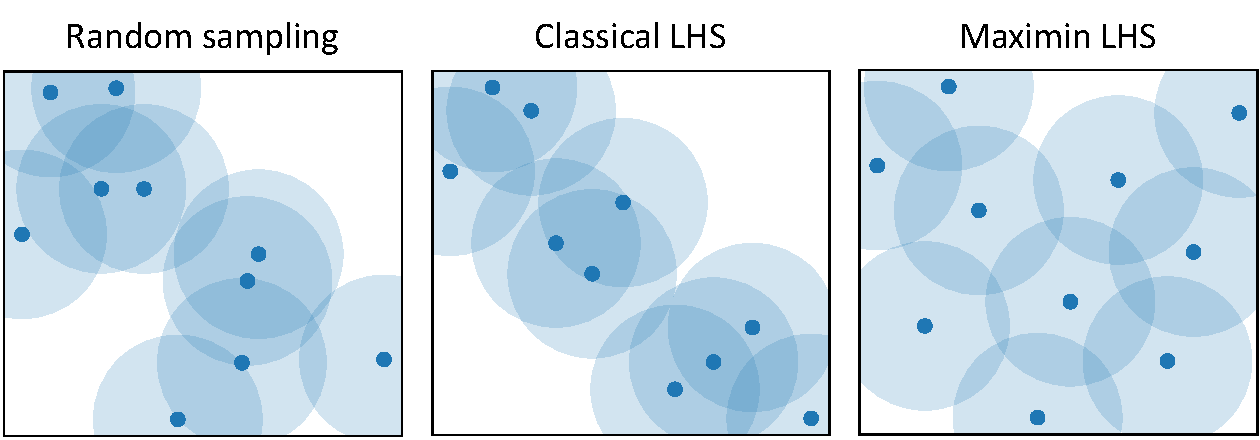
\includegraphics[width=0.47\textwidth]{sampling.pdf}
    \caption{{Space-filling sampling}. 10 random samples are used to illustrate three different sampling strategies: (a) simple random sampling (SRS), (b) classical LHS, and (c) maximin LHS.}
    \label{fig:lhs}
        \vspace{-0.5cm}
\end{figure}

In flow-based models, the data probability density $p_{\mathcal{X}}(x)$ and latent density $p_{\mathcal{Z}}(z)$ follow the principle of probability preservation based on the change of variable theorem, which means the probability and statistical information are preserved in the transformation process \citep{li2006probability}. To this end, the statistics of prior $p(\mathbf{z})$ are preservably propagated to the posterior density $p(\mathbf{x}|\mathbf{y})$. Inspired by this observation, we propose to better manipulate the prior samples by introducing a space-filling sampling for latent space $\mathbf z$ such that a diverse set of solutions are fully explored. 

Instead of simple random sampling (SRS), we propose to use Latin Hypercube Sampling (LHS) \citep{stein1987large, shields2016generalization}, which is a variance-reduced sampling method and often used for Monte Carlo integration \citep{mckay2000comparison} and simulation \cite{zhang2021modern}. As shown in Fig.~\ref{fig:lhs}, the LHS design shows better performance on space-filling than SRS, specifically the optimized LHS with maximin criteria, where an LHS design $\mathbf Z_n = \left\{\mathbf z_1, ...,\mathbf z_n \right\}$ that maximizes the minimum distance between all pairs of points,  
\begin{equation}
    \mathbf Z_n = \argmax_{\mathbf Z_n} \min\left\{d(\mathbf z_i, \mathbf z_j): i \neq j =1,...,m \right\} \label{eq:lhs}
\end{equation}
where $d$ is the Euclidean distance defined by $d(\mathbf z, \mathbf z^{\prime}) = \sum_{j=1}^{m} (\mathbf z_j-\mathbf z_j^{\prime})^2$. Unlike quasi-Monte Carlo (QMC) methods \citep{caflisch1998monte}, e.g., Sobol sequence, that are limited in high dimensional problem \citep{kucherenko2015exploring}, maximin LHS works well with strong space-filling property and variance reduction capability. 

\vspace{0.2cm}
\noindent {\bf \texttt{iPage}: Accelerating Inverse Learning Process}. We propose an efficient learning algorithm for solving inverse learning problems by leveraging \underline{i}ntelligent \underline{p}rior with \underline{a}ccelerated \underline{g}radient-based \underline{e}stimate, with exploratory latent space sampling, which consists of three core steps: training, inference, and localization process, as explained in Algorithm 1.  

\begin{algorithm}[h!]\label{algo:1}
\footnotesize
% \small
  \caption{\hspace{-0.1cm}: iPage algorithm}
\begin{algorithmic}[1]
\STATE{\bf Require}: training data $\left\{(\mathbf{x}_i, \mathbf{y}_i)_{i=1}^m \right\}$, invertible neural network model $f(\mathbf{x};\phi)$, prior distribution $p(\mathbf{x})$,  
% learning rates $\ell_{\psi}$ and $\ell_{\xi}$, $\tau$ in $I_{\rm SMILE}$, total prior samples $n$, total iterations $T$, implicit model $\mathcal{M}$
\vspace{0.1cm}
\STATE{// \bf \texttt{Training Process}}:
\vspace{0.1cm}
\STATE Initialize weight coefficients $\lambda_x$, $\lambda_y$ and $\lambda_z$  for each loss defined in Eq.~\eqref{eq:loss_y}-\eqref{eq:loss_x}  
\STATE Define an adaptive decay scheme for $\lambda_x$, $\lambda_y$ and $\lambda_z$ during the dynamic bi-directional training 
\STATE Minimize the total loss in Eq.~\eqref{eq:total_loss} via dynamic bi-directional training with gradient descent optimizer
\STATE Save the forward model $\hat{f}(\mathbf{x}; \phi^*)$ with the minimal $\ell_2$ loss 
\vspace{0.1cm}
\STATE{// \bf \texttt{Inference Process}}:
\vspace{0.1cm}
\STATE Generate a random sample $\mathbf{z}$ from latent space $p(\mathbf z)$ using optimized LHS with maximin criteria 
\STATE Compute the corresponding posterior sample $\hat{\mathbf{x}} = f^{-1}(\hat{\mathbf{y}}, \mathbf{z}; \phi)$ conditioned on the prior sample $\mathbf z$ and a specific observation $\hat{\mathbf{y}}$ through an invertible transformation 
\STATE Repeat sampling $\left\{\mathbf{z}_i \sim p(\mathbf{z}) \right\}_{i=1}^m$ to produce a number of posterior samples $\left\{\hat{\mathbf{x}}_i \sim \hat{p}({\mathbf{x}} | \hat{\mathbf{y}}) \right\}_{i=1}^m$ that follow the approximated posterior distribution $\hat{p}(\mathbf{x} | \hat{\mathbf{y}})$
\vspace{0.1cm}
\STATE{// \bf \texttt{Localization Process}}: 
\vspace{0.1cm}
\STATE Identify posterior samples $\left\{\hat{\mathbf{x}}_i \sim \hat{p}({\mathbf{x}} | \hat{\mathbf{y}}) \right\}_{i=1}^m$ as intelligent prior initialization to narrowing down the search space 
\STATE Compute the gradient $\mathbf{g}_i^{k}$ at the current $\hat{\mathbf{x}}_i$ using $\hat{f}_{\mathbf{y}}(\hat{\mathbf{x}}_i;{\phi}^*)$ in Eq.~\eqref{eq:gradient} using automatic differentiation. 
\STATE Localize these posterior samples precisely to exact solutions via gradient descent $\hat{\mathbf{x}}_{i}^{k+1} = \hat{\mathbf{x}}_i^{k} -\gamma ~ \mathbf{g}_i^{k}$
\STATE Return all possible exact inverse solutions $\mathbf{x}_i^{*}$
\end{algorithmic}
\end{algorithm}

\section{Experiments}
We start by demonstrating our proposed iPage method on a 2D sinewave function task and then extend our experiments to two artificial benchmark tasks. Finally, we introduce two real-world design problems from the field of quantum chemistry and additive manufacturing to illustrate the performance of learning complex high-dimensional inverse problems with practical objectives in natural sciences and engineering. 

\vspace{0.2cm}
\noindent{\bf Baseline Methods.} We provide five baseline methods: (1) Mixture density networks (MDN) \citep{bishop1994mixture}, which models the posterior distribution $p(\mathbf{x}|\mathbf{y})$ using a mixture of Gaussian models; (2) Invertible neural network (INN) \citep{ardizzone2018analyzing}, which is built on the flow-based model with latent variables to infer the completely posterior distribution; (3) Conditional invertible neural network (cINN) \citep{ardizzone2019guided, rombach2020network} which modifies INN framework by mapping the parameter space $\mathbf{x}$ and latent space $\mathbf{z}$ conditional on $\mathbf{y}$; (4) Conditional variational auto-encoder (cVAE) \citep{sohn2015learning}, which encodes $\mathbf{x}$ conditional on $\mathbf{y}$, into latent variables $\mathbf{z}$ based on the VAE framework, and (5) Neural-adjoint (NA) \cite{ren2020benchmarking}, which directly searches the global space
via surrogate-based optimization. To perform a fair comparison of all methods, we adjust neural network architectures such that all models have roughly the same number of model parameters. More information on benchmark details, baseline methods, invertible architectures, and datasets can be found in the Appendix.

\vspace{0.2cm}
\noindent{\bf Quantitative Metric.} We evaluate the true forward model $\Omega(\mathbf{x})$ at the generated inverse solutions $\mathbf{x}$ and measure the re-simulation error, which is defined as the mean squared error (MSE) to the target $\mathbf{y}^*$, $\mathcal{Q}_{\textup{re-sim}} = \mathbb{E}_{\mathbf{x}}\left\{ ||\Omega(\mathbf{x}) - \mathbf{y}^*||_2^2 \right\}$.
We apply this metric on two different scenarios: (1) solutions given 1000 different observations $\mathbf{y}_i^*, i=1,...,1000$, as shown in Table \ref{tab:1000_y}); and (2) solutions given a single specific observation $\mathbf{y}^*$, as shown in Table \ref{tab:1_y}.
\begin{table}[h!]
\vspace{-0.2cm}
% \begin{table}[!h] 
\footnotesize
% \scriptsize
\centering
\caption{Training dataset size, input/output dimensionality, and target observation $y^*$ for benchmark tasks and real-world applications.} 
\vspace{-0.2cm}
\label{tab:dataset}
\begin{tabular}{@{}ccccc@{}}
% \begin{tabular}{p{3cm}<{\centering}p{1cm}<{\centering}p{1cm}<{\centering}p{1.5cm}<{\centering}p{2.5cm}<{\centering}p{2.5cm}<{\centering}}
\toprule
Task        & Dim $\mathbf{x}$ & Dim $\mathbf{y}$ & Data size & Target  $y^*$ \\ \midrule
Sinewave        & 2     & 1         & 1.00E+04  & $y^*=1.2$     \\
Robotic Arm & 4     & 2         & 1.00E+04 & $y^*=[1.5,0]$     \\
Ballistics  & 4     & 1          & 1.00E+04 & $y^*=5$     \\
Crystal     & 6     & 1          & 5.00E+03  & $y^*=0.5$    \\ 
Architecture     & 1024     & 1          & 1.00E+05  & $y^*=1.0$    \\ 
\bottomrule
\end{tabular}
\end{table}

\vspace{0.2cm}
\noindent{\bf Datasets.} We focus on five datasets, including three benchmarks (sinewave, robotic arm, and ballistics) and two real-world (crystal and architecture design) problems. As shown in Table \ref{tab:dataset}, the first four tasks are low-dimensional problems and the last one, i.e., the architecture task is a high-dimensional design problem in image pixel levels. 

% Please add the following required packages to your document preamble:
% \usepackage{booktabs}
\begin{table*}[!htbp]
\footnotesize
% \scriptsize
\centering
\caption{Performance comparison of tested methods on five tasks given 1000 different observations $\mathbf{y}^*$). The re-simulation error measures how well the generated $\hat{\mathbf{x}}$ is conditioned on the observation $\mathbf{y}^*$. Each task is performed 50 times to obtain the standard deviation.}
\vspace{-0.2cm}
\label{tab:1000_y}
\begin{tabular}{@{}cccccc@{}}
% \begin{tabular}{p{2cm}<{\centering}p{2cm}<{\centering}p{2cm}<{\centering}p{2cm}<{\centering}p{2cm}<{\centering}p{2cm}<{\centering}}
\toprule
Method & Sinewave     & Robotic Arm     & Ballistics     & Crystal Design   & Architecture Design                          \\ \midrule
Mixture density networks (MDN)    & 0.17 $\pm$ 2.3e-4  & 0.018  $\pm$  1.1e-5  & 0.024 $\pm$ 1.3e-5 & 0.81 $\pm$   2.3e-2  & 1.74 $\pm$ 2.5e-1   \\
Invertible neural network (INN)    & 0.12 $\pm$ 7.8e-5  & 0.014  $\pm$  8.2e-6  & 0.019 $\pm$ 9.9e-6 & 0.49 $\pm$ 3.9e-2   & 0.88 $\pm$ 9.7e-2 \\
conditional INN (cINN)   & 0.11 $\pm$ 2.3e-4  & 0.009 $\pm$ 7.3e-6    & 0.421 $\pm$ 2.0e-5   & 0.35 $\pm$ 8.1e-2  & 0.76 $\pm$ 8.6e-2    \\
conditional VAE (cVAE)   & 0.13 $\pm$ 3.9e-4  & 0.021 $\pm$  9.0e-6   & 0.798 $\pm$ 1.8e-5   & 0.64 $\pm$ 5.6e-2  & 1.03 $\pm$ 1.8e-1   \\
Neural-Adjoint (NA)     & 0.006 $\pm$ 4.1e-6 & 0.008  $\pm$  8.8e-6  & 0.016 $\pm$ 1.4e-5   & 0.12 $\pm$  {\bf 4.4e-3}  & 0.71 $\pm$ 1.1e-1 \\ \midrule
% TuRBO   & 0.004 $\pm$ 2.9e-6 & {\bf 0.007}   $\pm$  9.2e-6 & 0.013 $\pm$ 2.1e-5   & 0.15 $\pm$ 5.1e-3     \\ \midrule
iPage (with maximin LHS)  & {\bf 0.002} $\pm$ {\bf 1.6e-6} & {\bf 0.006}  $\pm$  {\bf 4.2e-6}  & {\bf 0.011} $\pm$ {\bf 4.7e-6}   & {\bf 0.11} $\pm$ 4.5e-3  & {\bf 0.23} $\pm$ {\bf 1.2e-2} \\ \bottomrule
\end{tabular}
\end{table*}
\subsection{Illustrative Example: 2D Sinewave Function}
To test the capability of the iPage approach for solving inverse problems, we use a simple 2D sinusoidal function as a benchmark. The input parameters are $\mathbf{x} = [x_1, x_2]$ and the output is $y = \sin(3\pi x_1) + \cos(3\pi x_2)$. Due to its periodic nature, multiple solutions exist (theoretically infinite) given a specific observed $y^*$. 

\begin{figure}[h!]
    \centering
    \vspace{-0.2cm}
    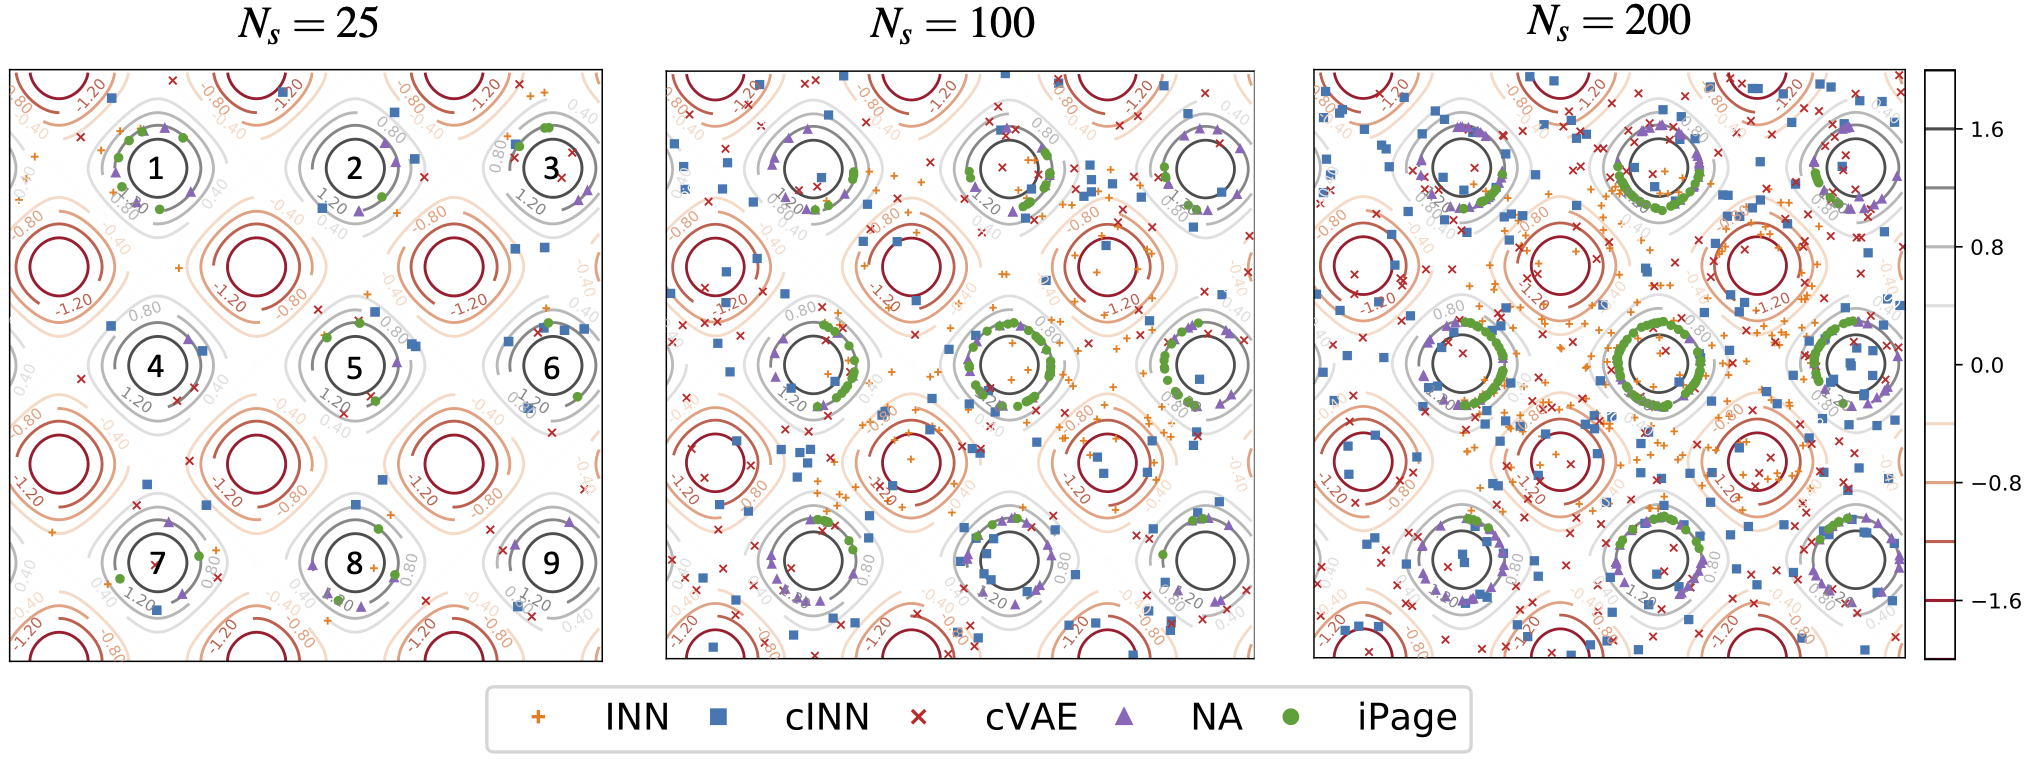
\includegraphics[width=0.48\textwidth]{four_v5.png}
    \caption{{Localization and exploration of inverse solutions for the 2D sinewave function}. Given a specific target $y^*=1.2$, there exits a multimodal disconnected solution space (labeled as 1-9 in the left panel). The inverse solution using four baseline methods (INN, cINN, cVAE, and NA) and iPage (with SRS) are illustrated and compared at different sampling counts ranging from 25 to 200.}
    \label{fig:sine9}
    \vspace{-0.2cm}
\end{figure}

For most of the existing baselines, this sinewave benchmark task remains a significant challenge task, specifically for obtaining accurate and diverse inverse solutions. An example of a fixed ${y}^*$ is shown in Fig.~\ref{fig:sine9}, where we compare our proposed methods to other baselines. We note that while the INN, cINN and cVAE methods are able to find some solutions within the local mode (marked by black circles labeled as 1-9), they fail to infer precise solutions. The NA method performs better in localizing to the globally optimal solution but fails to fully explore all possible solutions (e.g. missing mode 6). Our iPage method with simple random sampling (SRS) has the same difficulty (fails to capture modes 4 and 9) because the prior initialization fails to fully explore these local regions. Although this space exploration issue is mitigated by increasing the number of solutions as $N_s=100$, most of the localized solutions become concentrated on specific modes (e.g. modes 2, 5, and 6), with only limited solutions lie on the boundary modes (e.g. modes 9 and 3) for the case of $N_s=200$.

\begin{figure}[h!]
\vspace{-0.2cm}
    \centering
    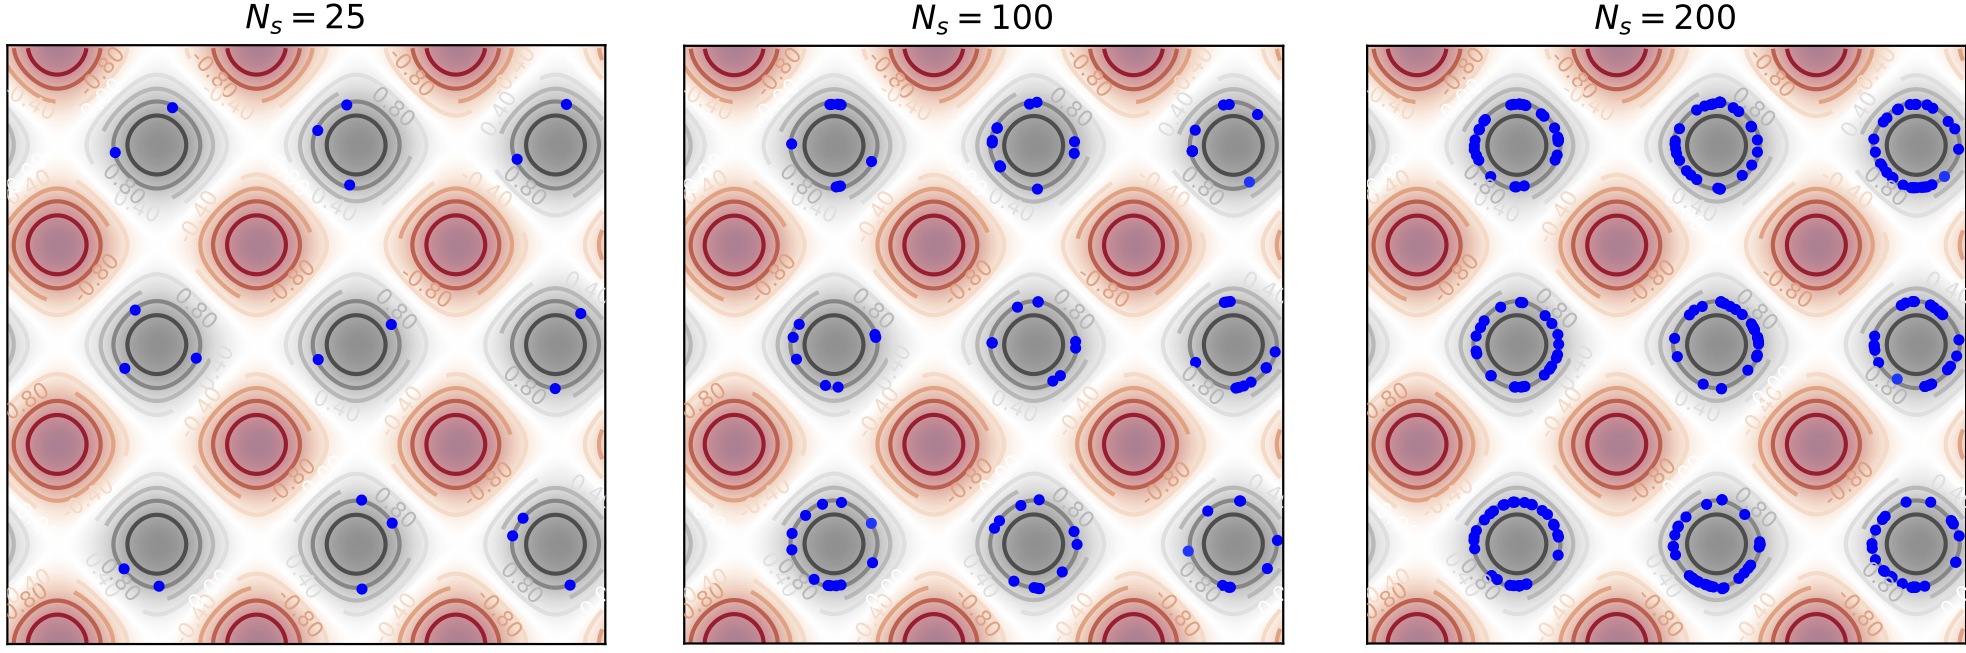
\includegraphics[width=0.48\textwidth]{new_four_v5.png}
    \caption{iPage (with mLHS) performance. Blue dots represent the final solutions, showing that our approach yields uniformly distributed solutions that capture all local modes.}
    \label{fig:iPage}
    % \vspace{-0.7cm}
\end{figure}

To better capture all potential solutions, we introduce the iPage method with maximin LHS which leverages space-filling sampling to achieve better results than the previous models (see Fig.~\ref{fig:iPage}). All 9 local modes are evenly covered by the optimal solutions even with a limited number of samples (e.g., $N_s=25$). The quantitative comparison for the two scenarios is shown in Table \ref{tab:1000_y} and \ref{tab:1_y} respectively. iPage (with mLHS) shows superior performance, especially for the re-simulation error variance. This provides a clear illustration of the advantages of using a space-filling sampling for space exploration and variance reduction. 
\begin{figure*}[!h]
    \centering
    \includegraphics[width=0.9\textwidth]{iPage2.pdf}
    \caption{{Two real-world design applications}: (Left) Crystal structure design problem in quantum chemistry and (Right) Architected materials design problem in additive manufacturing.}
    \label{fig:crystal}
    \vspace{-0.2cm}
\end{figure*}

\subsection{Artificial Benchmark Tasks}
Two artificial benchmark tasks used by \citet{ardizzone2018analyzing,ren2020benchmarking, kruse2021benchmarking} are further used to assess the iPage performance.

\vspace{0.2cm}
\noindent{\bf Robotic Arm Task.} This is a geometric benchmark that targets the inference of the position of a multi-jointed robotic arm from various configurations of its joints. The inverse problem is to obtain all possible solutions in the $\mathbf{x}$-space given any observed 2D positions $\mathbf{y}^*$. For the case of multiple different observations, iPage shows similar results to cINN and NA but with a slightly lower variance, as shown in 
Table \ref{tab:1000_y}. In the second setting (see Table \ref{tab:1_y}), iPage outperforms the other baselines with a much lower error and variance.

\vspace{0.2cm}
\noindent{\bf Ballistics Task.} In this case, cINN and cVAE fail to solve the problem with much larger errors than the others while NA and INN show similar performance to iPage (see Table \ref{tab:1_y}). In general, iPage outperforms the baselines in terms of overall stability and robustness.    

\begin{figure*}[h!]
    \centering
    \vspace{-0.1cm}
    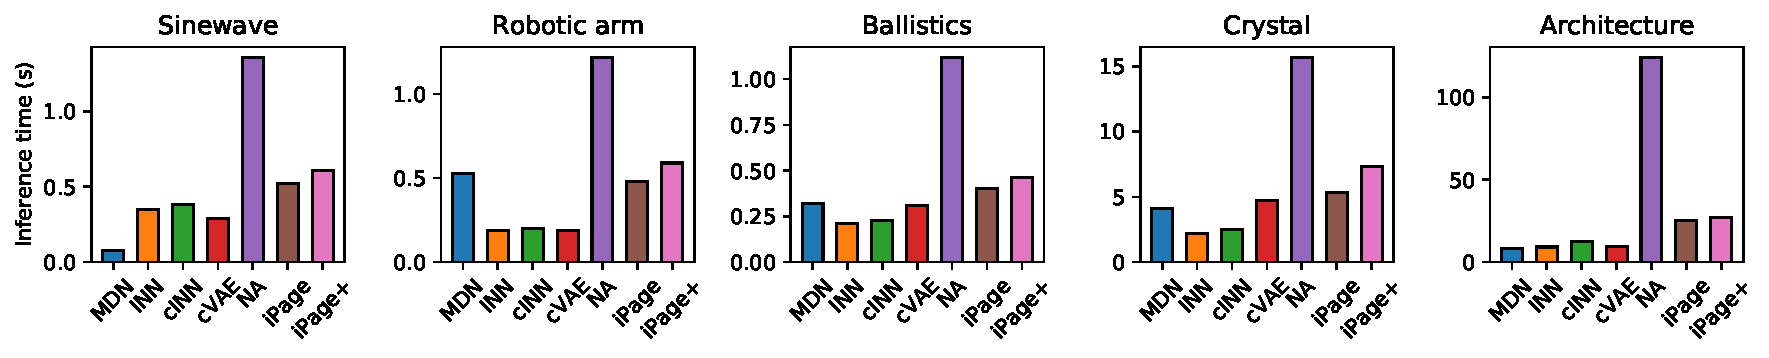
\includegraphics[width=0.9\textwidth]{time_comparsion_5.pdf}
    \vspace{-0.3cm}
    \caption{{Total time cost (inference and localization) for 1000 solutions}. The time-to-solution using iPage with other baselines on three benchmarks are compared side-by-side.}
    \label{fig:time}
        \vspace{-0.3cm}
\end{figure*}

\subsection{Real-world Applications}
We further demonstrate iPage's superiority in both natural sciences and engineering applications. 

\vspace{0.2cm}
\noindent{\bf Crystal Design Problem.} We apply our approach to a challenging real-world application in materials design, specifically one for modeling the electronic properties of complex metal oxides. 
Quantum chemistry simulations are performed to simulate these materials under perturbation and obtain their resulting electronic properties such as the band gap. Here, we tackle the inverse problem of the band gap to strain mapping for the case of the SrTiO\textsubscript{3} perovskite oxide, which is otherwise intractable to obtain from quantum chemistry. This can be an exceptionally difficult problem due to the complex underlying physics, and the high degree of sensitivity of the band gap to the lattice parameters, requiring very accurate predictions for the generated structures to succeed. 

% Please add the following required packages to your document preamble:
% \usepackage{booktabs}
\begin{table*}[!h] 
\footnotesize
% \scriptsize
\centering
\caption{Performance comparison of tested methods on five tasks for 1000 solutions conditioned on a specific observation $\mathbf{y}^*$. We repeat 50 times to obtain the standard deviation for each case.} 
% We measure the re-simulation error on 1000 solutions $\mathbf{x}$ given $\mathbf{y}^*$. }
\vspace{-0.2cm}
\label{tab:1_y}
\begin{tabular}{@{}cccccc@{}}
% \begin{tabular}{p{2.5cm}<{\centering}p{2.5cm}<{\centering}p{2.5cm}<{\centering}p{2.5cm}<{\centering}p{3cm}<{\centering}p{2.5cm}<{\centering}}
\toprule
Method & Sinewave     & Robotic Arm     & Ballistics     & Crystal Design  & Architecture Design \\ \midrule
Mixture density networks (MDN)    & 0.22 $\pm$ 5.1e-4 & 0.023 $\pm$ 2.3e-5  & 0.041 $\pm$ 2.9e-5 & 0.84 $\pm$ 3.3e-2   & 1.81 $\pm$ 2.0e-1\\
Invertible neural network (INN)    & 0.19 $\pm$ 9.3e-5  & 0.015 $\pm$ 4.7e-5  & {0.024} $\pm$ 1.9e-5 & 0.57 $\pm$ 4.7e-2  & 0.83 $\pm$ 9.1e-2 \\
conditional INN (cINN)   & 0.16 $\pm$ 5.0e-4  & 0.032 $\pm$ 3.1e-5   & 0.652 $\pm$ 4.3e-5   & 0.42 $\pm$ 8.8e-2 & 0.82 $\pm$ 8.5e-2   \\
conditional VAE (cVAE)   & 0.25 $\pm$ 7.0e-4  & 0.021 $\pm$ 5.6e-5   & 0.912 $\pm$ 3.2e-5   & 0.70 $\pm$ 9.0e-2  & 1.20 $\pm$ 1.7e-1 \\
Neural-Adjoint (NA)     & 0.011 $\pm$ 9.1e-6 & 0.012 $\pm$ 4.8e-5  & 0.031 $\pm$ 4.7e-5   & {0.15} $\pm$ 6.6e-3  & 0.79 $\pm$ 9.3e-2 \\ \midrule
% TuRBO  & 0.007 $\pm$ 7.9e-6 & 0.009 $\pm$ 4.7e-5 & 0.026 $\pm$ 4.3e-5   & 0.18 $\pm$ 5.1e-3  & 0.18 $\pm$ 5.1e-3  \\ \midrule
iPage (with maximin LHS) & {\bf 0.004} $\pm$ {\bf 2.1e-6} & {\bf0.008} $\pm$ {\bf7.6e-6}  & {\bf 0.023} $\pm$ {\bf 8.9e-6}   & {\bf0.14} $\pm$ {\bf 2.2e-3}  & {\bf 0.22} $\pm$ {\bf 1.2e-2}  \\ \bottomrule
% \vspace{-0.5cm}
\end{tabular}
\end{table*}

Strain is represented by changes in the crystal lattice constants and angles, $a, b, c, \alpha, \beta, \gamma$, which serve as the hidden parameters $\mathbf{x}$. The target property y is the electronic band gap. 5000 samples were used for training where band gaps were obtained using quantum chemistry, representing the forward process. Additional details can be found in the appendix. We provide this dataset as a novel benchmark for computational chemistry, the first such example for solid state materials. We herein select an arbitrary target of 0.5 eV to generate our structures and compare the performance of our model with the existing ones. The new crystals are generated for each model and the band gaps are then computed using quantum chemistry for validation (see Fig.\ref{fig:crystal}). The performance of our approach was found to be significantly better than the baseline invertible models, INN, cINN, and cVAE, as shown in Table \ref{tab:1000_y} and \ref{tab:1_y}. By comparison, the INN, cINN, and cVAE models are consistently off the target by a far greater degree, with a deviation of 0.5-1.0 eV. The generated lattice parameters do not deviate much from the equilibrium values (see Fig.~\ref{fig:crystal}) and thus the results are unsurprisingly poor. Based on these observations and the magnitude of the deviations, it is unlikely these methods will provide useful results even with further training data provided. Only the NA method provides results with similar performance to iPage, though at a significantly greater computational cost. Furthermore, the NA method encounters difficulties for problems with a larger dimensionality in the parameter space. 

\vspace{0.2cm}
\noindent{\bf Architecture Materials Design Problem.} Architected materials on length scales from nanometers to meters are desirable for diverse applications \citep{mao2020designing}. Recent advances in additive manufacturing have made mass production of complex architected materials technologically and economically feasible. This task aims to find the optimal material layout by searching the design space (1024 dimensions) given a specific target mechanical property (see more details in the Appendix). The input is the pixel matrix for the element, and the output is the effective Young's modulus. We use this example to demonstrate that iPage can well scale to high-dimensional problems, e.g., pixel-level images, and outperform the other baseline methods. 

\subsection{Computational Cost Comparison}
% \vspace{0.2cm}
% \noindent{\bf Computational Cost Comparison}
We have demonstrated that the iPage can precisely localize the exact inverse solutions and quantitatively outperform INN, cINN, cVAE and MDN methods on five tasks. The NA method has advantages in learning accuracy but shows an obvious drawback of large computational costs compared to the other models. Fig.~\ref{fig:time} shows the total time cost including the inference and localization process on five tasks using one NVIDIA V100 GPU. Due to the invertible architecture, INN and cINN are efficient at sampling the posterior distributions. The time cost of iPage is slightly higher than INN, cINN and cVAE but still significantly lower than NA even though gradient descent is employed (few steps in local search). 

\section{Conclusion}
In this work, we develop an efficient inverse learning approach that utilizes posterior samples to accelerate the localization of all inverse solutions via gradient descent. To fully explore the parameter space, variance-reduced sampling strategies are imposed on the latent space to improve space-filling capability. Multiple experiments demonstrate that our approach outperforms the baselines and significantly improves the accuracy, efficiency, and robustness for solving inverse  problems, specifically in complex natural science and engineering design applications.  One current limitation is the efficiency of space-filling sampling in high-dimensional spaces. 
% Additional computational cost is required compared with simple random sampling, specifically in high-dimensional spaces. 
Future work will aim to improve sampling efficiency by leveraging scalable numerical algorithms. Also, we plan to apply the iPage method to broader topics in safe and robust AI, e.g., safe decision-making with Bayesian optimal experimental design \cite{zhang2021scalable}, and privacy defense in federated learning \cite{li2022auditing}.  

\bibliography{aaai23}
% \bibliographystyle{unsrt}
% \bibliographystyle{plain}

\appendix
\section{Appendix}
\section{Baseline Inverse Methods}
\label{Baseline Methods}
Here we provide more technical details about the baseline inverse methods used in our paper. 
\subsection{Invertible Neural Network (INN)}
This inverse model is our fundamental baseline, which is based on the invertible architecture with affine coupling layers. The basic idea is to define a forward L2 loss for fitting the y-prediction to the training data 
\begin{equation}
    \mathcal{L}_{\mathbf{y}} = ||\mathbf{y}-\mathbf{y}_t||_2^2
\end{equation}
where $\mathbf{y}_t$ is the true output. Then a backward MMD loss $\mathcal{L}_{\mathbf{z}}=\textup{MMD}(\mathbf{z})$ is used to fit the probability distribution of latent variable $p(\mathbf{z})$ to a standard Gaussian distribution $\mathcal{N}(\mathbf{0}, \mathbf{I})$. Therefore, a total loss is defined with weighting factors $\lambda_{\mathbf{y}}$ and $\lambda_{\mathbf{z}}$:
\begin{equation}
    \mathcal{L} = \lambda_{\mathbf{y}} \mathcal{L}_{\mathbf{y}} + \lambda_{\mathbf{z}} \mathcal{L}_{\mathbf{z}}
\end{equation}

Kruse et al.\cite{kruse2021benchmarking} proposed an alternative way to train the INNs with a maximum likelihood loss. This is achieved by assuming $\mathbf{y}$ to be normally distributed around the true values $\mathbf{y}_t$ with very low variance $\sigma^2$: 
\begin{equation}
    \mathcal{L} = \frac{1}{2} \left(\frac{1}{\sigma^2} \cdot (\mathbf{y} - \mathbf{y}_t)^2 + \mathbf{z}^2 \right) - \log |\textup{det} J_{\mathbf{x} \mapsto [\mathbf{y},\mathbf{z}]} |
\end{equation}
% We use the implementation introduced by \cite{ardizzone2018analyzing} with the GitHub link: \url{https://github.com/VLL-HD/analyzing_inverse_problems}. For the neural spline flows, we use the implementation developed by \cite{durkan2019neural} at \url{https://github.com/bayesiains/nflows}. 

\subsection{Conditional Neural Network (cINN)}
The INN model may have a challenge when the dimensionality of $\mathbf{x}$ is significantly larger than $\mathbf{y}$, for example, in image-based inverse problems. Thus, instead of training INN to predict $\mathbf{y}$ and $\mathbf{x}$ with additional latent variable $\mathbf{z}$, cINN transforms $\mathbf{x}$ directly to a latent representation $\mathbf{z}$ conditional on the observation $\mathbf{y}$. This is achieved by using $\mathbf{y}$ as an additional input to each affine coupling layer in both the forward and backward processes. We can also use maximum likelihood to train cINN as 
\begin{equation}
    \mathcal{L} = \frac{1}{2} \cdot \mathbf{z}^2 - \log \left|\textup{det} J_{\mathbf{x} \mapsto \mathbf{z}} \right|
\end{equation}
We use the original authors' implementation in both invertible architecture \cite{kruse2021benchmarking}. 

\subsection{Conditional Variational Autoencoder (cVAE)}
The conditional variational autoencoder uses the evidence lower bound and encodes the $\mathbf{x}$ into Gaussian distributed random latent variable $\mathbf{z}$ conditioned on $\mathbf{y}$. The forward training process utilizes the L2 loss to achieve a good reconstruction of the original input $\mathbf{x}$, and the backward process is to solve $\mathbf{x}$ which is decoded from random samples that are drawn from latent space $\mathbf{z}$ conditioned on $\mathbf{y}$. The loss function is defined as 
\begin{equation}
    \mathcal{L} = \alpha \cdot (\mathbf{x}-\hat{\mathbf{x}})^2 - \frac{1}{2} \cdot \beta \cdot (1+\log \mathbf{\sigma}_{z} - \mathbf{\mu}_z^2 -\mathbf{\sigma}_z)
\end{equation}
We use the code implemented by \cite{ma2019probabilistic} for this method. 

\subsection{Mixture Density Network (MDN)}
The mixture density network can model the inverse problem but it is not an invertible model. MDN uses $\mathbf{y}$ as an input and predicts the parameters $\mathbf{\mu}_x, \Sigma_x^{-1}$ of a Gaussian mixture model $p(\mathbf{x}|\mathbf{y})$. We train the MDN model by maximizing the likelihood of the training data with the following loss function:
\begin{equation}
    \mathcal{L} = \frac{1}{2} \cdot \left( \mathbf{x} \mathbf{\mu}_x^{\top} \cdot \Sigma_x^{-1} \cdot \mathbf{x} \mathbf{\mu}_x \right) - \log |\Sigma_x^{-1}|^{1/2}
\end{equation}
We implemented this method according to \cite{bishop2006pattern}.

\subsection{The Neural-Adjoint (NA) Method}
The NA method, different from the other methods, uses a deep neural network as a surrogate (i.e., approximation) for the forward model and then uses backpropagation with respect to the input variable to search for good inverse solutions \cite{ren2020benchmarking}. The authors \cite{ren2020benchmarking} propose an alternative metric that quantifies the expected minimum error by drawing a sequence of $z$ values of length T, denoted $Z_T$, which is given as:
\begin{equation}
    r_T = \mathbb{E}_{(x,y) \sim \mathcal{D}, Z_T \sim \Omega} \left[ \min_{z \in Z_T} [ \mathcal{L}(\hat{y}(z)),y]\right]
\end{equation}
where $Z_T$ is a sequence of length $T$ drawn from a distribution $\Omega$, which characterizes the expected loss of an inverse problem as a function of the number of samples of $z$ for each target $y$. They claim that solving inverse problems strongly depends on $T$. Additionally, to narrow the stochastic search space in the model input domain, a boundary loss is proposed to ensure the NA identifies solutions that are within the training data domain, which is given by:
\begin{equation}
    \mathcal{L}_b = \texttt{ReLU}(|\hat{x} - \mu_x| - \frac{1}{2}R_x)
\end{equation}
where $R_x$ is the bounded range of input domain, $\mu_x$ is the mean of the training data, and $\texttt{ReLU}$ is the conventional nonlinear activation function. For this method, we use the implementation provided by the authors \cite{ren2020benchmarking} at \url{https://github.com/BensonRen/BDIMNNA}. 


\section{Artificial Benchmark Tasks: Additional Details}
Two benchmark tasks that have been used by \citep{ardizzone2018analyzing,ren2020benchmarking, kruse2021benchmarking} are also employed to assess the algorithm performance. 

\subsection{Robotic arm task}
This is a geometric benchmark example that targets the inference of the position of a multi-jointed robotic arm from various configurations of its joints. There are four input parameters: starting height $x_1$, three joint angles $x_2$, $x_3$, and $x_4$ in the forward model. The output is the arm's position $[y_1, y_2]$ as: 
% $y_1 = l_1\sin(x_2) + l_2\sin(x_3-x_2) + l_3\sin(x_4-x_2-x_3) + x_1  $ and $y_2 = l_1\cos(x_2) + l_2\cos(x_3-x_2) + l_3\cos(x_4-x_2-x_3) $
    % $$y_1 = l_1\sin(x_2) + l_2\sin(x_3-x_2) + l_3\sin(x_4-x_2-x_3) + x_1 $$ 
    % $$y_2 = l_1\cos(x_2) + l_2\cos(x_3-x_2) + l_3\cos(x_4-x_2-x_3) $$
\begin{equation}
\begin{aligned}
    y_1 &= l_1\sin(x_2) + l_2\sin(x_3-x_2) \\
    &+l_3\sin(x_4-x_2-x_3) + x_1  
\end{aligned}
\end{equation}
\begin{equation}
\begin{aligned}
    y_2 &= l_1\cos(x_2) + l_2\cos(x_3-x_2) \\
    &+ l_3\cos(x_4-x_2-x_3)
\end{aligned}
\end{equation}
where $l_1=0.5$, $l_2=0.5$ and $l_3=1$ in this case. The parameters $\mathbf{x}$ have a Gaussian prior $\mathbf{x} \sim p(\mathbf{x}) = \mathcal{N}(0, \sigma^2 \cdot \mathbf{I})$ with $\sigma^2 = [\frac{1}{16}, \frac{1}{4}, \frac{1}{4},\frac{1}{4}]$. The inverse problem is to obtain all possible solutions in the $\mathbf{x}$-space given any observed 2D positions $\mathbf{y}^*$. 

\subsection{Ballistics task}
The forward process in this example can be interpreted as an object being thrown from position $(x_1, x_2)$ with angle $x_3$ and initial velocity $x_4$ and the output is the object's final position on the horizontal axis $y = T_1(t^*)$ where $t^*$ is the solution of $T_2(t^*)=0$. The object's trajectory $\mathbf{T}(t)$ can be computed analytically as follows:
\begin{equation}
    T_1(t) =x_1 - \frac{v_1 m}{k}\cdot \left( \exp\left(-\frac{kt}{m}\right)-1\right)
\end{equation}
\begin{equation}
\begin{aligned}
    T_2(t) &=x_2 - \frac{m}{k^2} \cdot ( \left( gm + v_2 k \right) \\ &\cdot \left(\exp\left(-\frac{kt}{m} \right)-1 \right) + gtk )
\end{aligned}
\end{equation}
% \begin{equation}
% \begin{aligned}
%     T_1(t) &=x_1 - \frac{x_4\cdot \cos(x_3) \cdot m}{k}\cdot \\ & \left( \exp\left(-\frac{kt}{m}\right)-1\right)
% \end{aligned}
% \end{equation}
% \begin{equation}
% \begin{aligned}
%     T_2(t) & =x_2 - \frac{m}{k^2}\cdot \left( gm + x_4\cdot \sin(x_3) \cdot k \cdot  \\ & \left(\exp\left(-\frac{kt}{m}\right)-1 \right) + gtk\right).
% \end{aligned}
% \end{equation}

Given gravity $g$, object mass $m$ and air resistance $k$. $v_1=x_4 \cdot \cos(x_3)$ and $v_2 = x_4 \cdot \sin(x_3)$ are the horizontal and vertical velocity respectively. The prior distributions are defined as $x_1 \sim \mathcal{N}(0, \frac{1}{4})$, $x_2 \sim \mathcal{N}(\frac{3}{2}, \frac{1}{4})$, $x_3 \sim \mathcal{U}(9^{\circ},72^{\circ})$ and $x_4 \sim \textup{Poisson}(15)$. 


\section{Real-World Applications: Additional Details}

\subsection{Crystal design problem}
\paragraph{Background}
We apply our approach to a challenging real-world application in materials design, specifically for modeling the electronic properties of complex metal oxides. Metal oxides can exhibit significant changes in their electronic and magnetic properties in the presence of external perturbations such as strain, and electric and magnetic fields, with major implications for the design of neuromorphic and quantum devices \cite{RN6466, RN6431, RN6467}.


\paragraph{Methods for Crystal Prediction Experiment}
Lattice constants and angles $a$, $b$, $c$, $\alpha$, $\beta$, $\gamma$ were sampled uniformly within a range of 10\% deviation from the equilibrium crystal parameters: $a=b=c=3.914$ \AA ~and  $\alpha=\beta=\gamma=90^{\circ}$. Within the perturbed ranges ( 10\% of equilibrium value) in the lattice constants of the training data, the band gaps of the crystals were found to vary between 0 to 2.8 eV, representing a very wide range in energies. For reference, the band gap of the unperturbed crystal computed at this level of theory is 2.37 eV. In our experiment, we select an arbitrary target of 0.5 eV to generate our structures and compare the performance of our model with the existing ones. 

A total of 5000 structures were generated and band gaps were obtained using density functional theory (DFT). The distribution of calculated band gaps in the dataset is shown in Fig. \ref{fig:crystal2}. The DFT calculations were performed with the Vienna Ab Initio Simulation Package (VASP) \cite{RN138, RN144}. The Perdew-Burke-Ernzerhof (PBE)\cite{RN145} functional within the generalized-gradient approximation (GGA) was used for electron exchange and correlation energies. The projector-augmented wave method was used to describe the electron-core interaction \cite{RN141, RN138}. The on-site Coulomb interaction was included using the DFT+U method by Dudarev, et al.\cite{RN147} in VASP using a Hubbard parameter U = 4 eV for the Ti based on previous studies \cite{RN6481, RN6480}.  A kinetic energy cutoff of 500 eV was used. All calculations were performed with spin polarization. The Brillouin zone was sampled using a Monkhorst-Pack scheme with an $8\times8\times8$ grid \cite{RN148}. 

\begin{table*}[!h] 
\centering
\caption{Generated lattice parameters for the crystal band gap experiment for $y^*=0.5$ eV} 
\label{tab:crystal}
\begin{tabular}{@{}ccccccc@{}}
% \begin{tabular}{p{2cm}<{\centering}p{1.5cm}<{\centering}p{1.5cm}<{\centering}p{1.5cm}<{\centering}p{1.5cm}<{\centering}p{1.5cm}<{\centering}p{1.5cm}<{\centering}}
\toprule
Method    & a     & b     & c     & $\alpha$       & $\beta$       & $\gamma$       \\ \midrule
iPage 1   & 4.412 & 3.524 & 3.923 & 94.132  & 95.124  & 106.975 \\
iPage 2   & 3.621 & 4.125 & 4.692 & 85.133  & 102.299 & 77.432  \\
INN   & 4.134 & 3.931 & 4.016 & 92.728  & 89.834  & 92.207  \\
cINN  & 3.972 & 3.952 & 3.923 & 93.357  & 89.815  & 90.199  \\
cVAE  & 4.073 & 4.133 & 4.126 & 90.152  & 89.128  & 91.298  \\
NA    & 3.510 & 4.602 & 4.825 & 94.988  & 95.016  & 103.775 \\ \bottomrule
\end{tabular}
\end{table*}

\begin{figure}[h!]
    \centering
    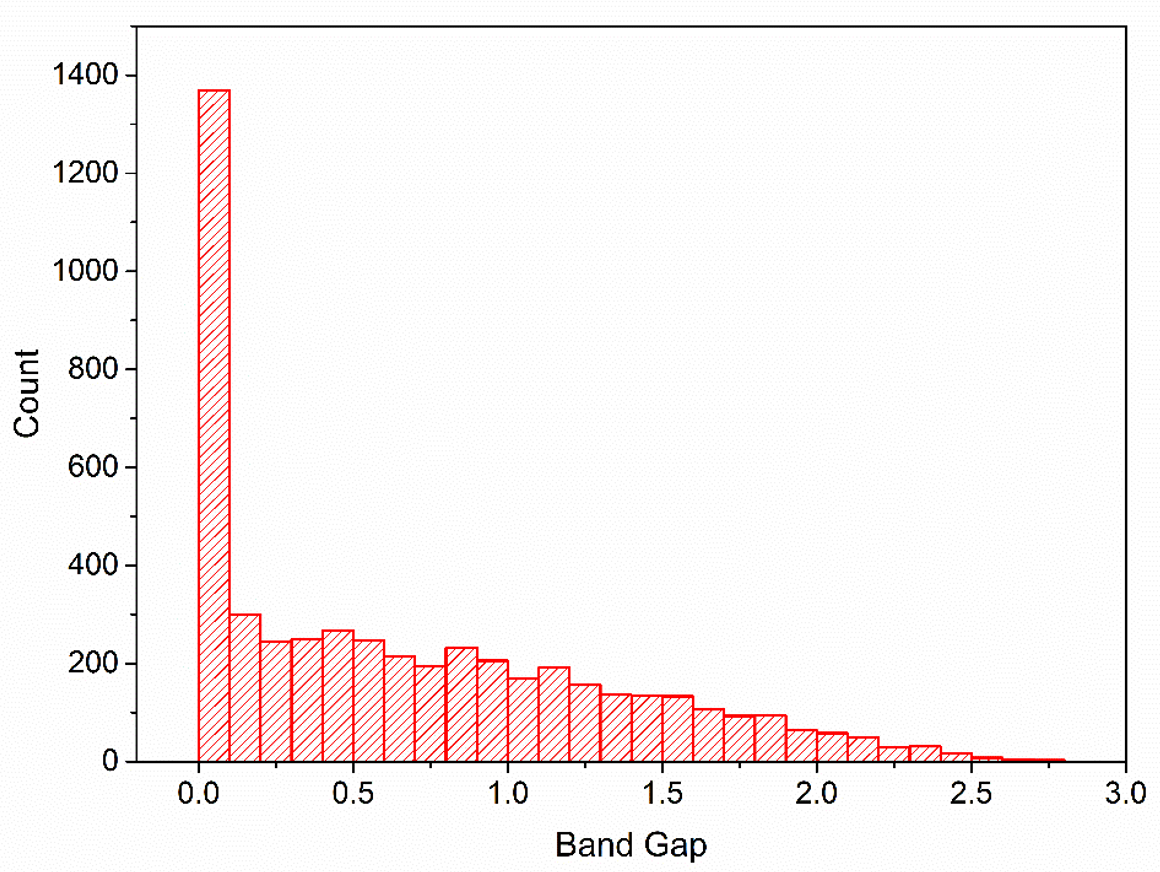
\includegraphics[width=0.4\textwidth]{crystal_dis.png}
    % \vspace{-0.5cm}
    \caption{Distribution of calculated band gaps in the dataset.}
    \label{fig:crystal2}
    % \vspace{-0.2cm}
\end{figure}

\begin{table*}[!h]  
% \footnotesize
\centering
\caption{Hyperparameter settings for each benchmark task} 
\label{tab:setting}
\begin{tabular}{@{}cccccc@{}}
% \begin{tabular}{p{4cm}<{\centering}p{1.5cm}<{\centering}p{1.5cm}<{\centering}p{1.5cm}<{\centering}p{1.5cm}<{\centering}p{1.5cm}<{\centering}}
\toprule
Parameters                              & Sinewave  & Robotic Arm & Ballistics  & Crystal  & Architecture  \\ \midrule
Number of invertible blocks             & 4         & 6           & 6           & 4  & 6       \\
Number of fully connected (fc)   layers & 3         & 3           & 3           & 3  & 3       \\
Number of neurons in each fc            & 128       & 256         & 256         & 64  & 512       \\
Activation function in each fc          & ReLU      & Leakly ReLU & Leakly ReLU & ReLU  & ReLU    \\
Optimizer for invertible training                               & Adam      & Adam        & Adam        & Adam & Adam      \\
Optimizer for localization                               & Adam      & Adam        & Adam        & Adam & Adam     \\
Batch size                              & 1024      & 512         & 512         & 256  & 1024      \\
Number of training epoch                & 1000      & 500         & 500         & 1000 & 10000     \\
Learning rate (decay) for invertible training                   & 1e-3-1e-5 & 1e-2-1e-4   & 1e-2-1e-4   & 1e-3-1e-5 & 1e-3-1e-5 \\
Learning rate for localization                   & 1e-3 & 5e-3   & 5e-3   & 1e-3 & 1e-4 \\ \bottomrule
\end{tabular}
\end{table*}

\subsection{Architected materials design problem}
\paragraph{Background}

Architected materials on length scales from nanometers to meters are widely used fro many practical applications \cite{mao2020designing}. Controlling material architecture a complex interplay of topology, material distribution, and constituent material behavior is a powerful way to create materials with tailored and often unprecedented properties. We, therefore, envision a shift towards a materials-by-design approach that takes advantage of rapid advancements in material synthesis, and in particular additive manufacturing, to produce novel material systems across many length scales and with multiple functionalities. Examples of interest include mechanical, seismic, and acoustic meta-materials, additively manufactured lattices and foams, nanostructured materials, optimized architectures, and design algorithms, materials for extreme environments, and natural architected materials. 

\paragraph{Data generation}
We generate the data from topology optimization approaches \cite{bendsoe2013topology}. Based on the symmetric properties, topology optimization is an effective way to obtain the desired architecture given a specific elastic property, e.g., Young's Modulus $E$. The input is the pixel matrix for the element of an architected material, and the output is the effective mean Young's modulus of the corresponding architected materials. The size of the dataset is one million configurations, including different groups with various porosities, typically ranging from 0.25 to 0.75. 



\section{Details of Hyperparameter Settings}
In Table \ref{tab:setting}, we provide a summary of the hyperparameter settings, including the neural network model, number of training epochs, batch size, invertible architectures, optimizer, learning rate decay and etc, for each benchmark task. 

% Please add the following required packages to your document preamble:
% \usepackage{booktabs}
\end{document}

